\newcommand*{\DocType}{scrartcl}
\newcommand*\ClassList{scrartcl,article}

\documentclass[\DocType, abstract=on, paper=a4, fontsize=11pt]{generalclass}

% Packages
\usepackage[a4paper]{geometry}
\usepackage[english]{babel}
\usepackage[utf8]{inputenc}
\usepackage[automark]{scrpage2}
%\usepackage[automark, headsepline,footsepline]{scrlayer-scrpage}
\usepackage{xargs} % Use more than one optional parameter in a new commands
\usepackage[pdftex,dvipsnames]{xcolor}  % Coloured text etc.
\usepackage{graphicx} % Images etc.
\usepackage{amssymb}
\usepackage{amsmath}
\usepackage{amsthm} % better theorems
\usepackage{mathtools} % e.g ":=" 
\usepackage[super]{nth} % use superscripts for 1st, 2nd, 3rd
\usepackage[sort, numbers, square]{natbib} % citeauthor, citet
\usepackage{physics} % norm
\usepackage{enumitem} % changing enumeration styles
\usepackage{gensymb} % degree
\usepackage{booktabs} % nice table separators
\usepackage{tabularx} % better tables, X column
\usepackage{caption} % change style of figure 
\usepackage{subcaption} % subfigures
\usepackage{tikz} % for pgfplots
\usepackage{tkz-euclide} % for coordinate system etc.
\usepackage{pgfplots} % plotting data
\usepackage[section]{placeins} % place figures in the sections they appear in
\usepackage[colorinlistoftodos,prependcaption,textsize=tiny]{todonotes}
\usepackage{parskip} % space between paragraphs instead of indent
\usepackage{csquotes} % autmatic left quotation marks
\usepackage{aliascnt} % alias counts
\usepackage[outline]{contour} % bold arrows
\usepackage{algorithmic}
\usepackage{bbm} % double struck numbers
\usepackage{tikz-cd} % commutative diagrams
\usepackage[activate=true,final,tracking=true,kerning=true,factor=1100,stretch=10,shrink=10]{microtype} % even better line spacing
\usepackage{xr-hyper} 
\usepackage[pagebackref, pdftex, colorlinks=true, linkcolor=blue, citecolor=blue]{hyperref}
\usepackage[capitalize,nameinlink,noabbrev]{cleveref} % better "\autoref"

% use " as left quotation mark
\MakeOuterQuote{"}

% Avoid cref double parantheses for equations
\creflabelformat{equation}{#2\textup{#1}#3}
	
\usetikzlibrary{positioning, arrows, matrix}
%\usetikzlibrary{external}
%\tikzexternalize[prefix=out/]
%\makeatletter
%\renewcommand{\todo}[2][]{\tikzexternaldisable\@todo[#1]{#2}\tikzexternalenable}
%\makeatother

\rehead{right even}

\makeatletter

\let\oldtheequation\theequation
\renewcommand\tagform@[1]{\maketag@@@{\ignorespaces#1\unskip\@@italiccorr}}
\renewcommand\theequation{(\oldtheequation)}


% Multiple abstracts
\newenvironment{polyabstract}[1]
{\renewcommand{\abstractname}{#1}\begin{abstract}}
	{\end{abstract}}

% Define new environment for problem
\newaliascnt{problem}{equation}
\newenvironment{problem}%
{\begin{equation*}\refstepcounter{problem}}
{\eqno \hbox{\@eqnnum}\end{equation*}\@ignoretrue}

\makeatother

% Set custom cref names
\crefname{problem}{Problem}{Problem}

% Rename autorefnames
\addto\extrasenglish{
	\renewcommand{\sectionautorefname}{Section}
	\renewcommand{\subsectionautorefname}{Section}
	\renewcommand{\subsubsectionautorefname}{Section}
}

% Captions for figures
\captionsetup{justification=raggedright, format=plain, font=small,labelfont=bf}


\newcommandx{\unsure}[2][1=]{\todo[linecolor=orange,backgroundcolor=orange!25,bordercolor=orange,#1]{#2}}
\newcommandx{\Todo}[2][1=]{\todo[linecolor=yellow,backgroundcolor=yellow!25,bordercolor=yellow,#1]{#2}}
\newcommandx{\info}[2][1=]{\todo[linecolor=green,backgroundcolor=green!25,bordercolor=green,#1]{#2}}

% Centered, equally spaced columns
\newcolumntype{Y}{>{\centering\arraybackslash}X} % centered equidistant columns

\setenumerate{label=(\arabic*),itemsep=0mm} % enumerate labeling and line distance
\renewcommand{\baselinestretch}{1.1} % line distance
\allowdisplaybreaks % Make big equations breakable

% add possibility to increase verticle spacings in matrices
\makeatletter
\renewcommand*\env@matrix[1][\arraystretch]{%
	\edef\arraystretch{#1}%
	\hskip -\arraycolsep
	\let\@ifnextchar\new@ifnextchar
	\array{*\c@MaxMatrixCols c}}
\makeatother

\newcommand{\cX}{\mathcal{X}}
\newcommand{\cY}{\mathcal{Y}}
\newcommand{\cL}{\mathcal{L}}
\newcommand{\cH}{\mathcal{H}}
\newcommand{\cV}{\mathcal{V}}
\newcommand{\cA}{\mathcal{A}}
\newcommand{\cF}{\mathcal{F}}
\newcommand{\R}{\mathbb{R}}

\newcommand{\fL}{\mathfrak{L}}
\newcommand{\fH}{\mathfrak{H}}
\newcommand{\fV}{\mathfrak{V}}

\newcommand{\dK}{\mathbb{K}}

\newcommand{\closure}{\mathrm{\mathbf{cl}}}

\newcommand{\bGamma}{\mathbf{\Gamma}}

\DeclareMathOperator*{\argmax}{arg\,max}
\DeclareMathOperator*{\argmin}{arg\,min}
\newcommand{\T}{\mathrm{T}}


\newtheoremstyle{break}% name
{\topsep}%         Space above, empty = `usual value'
{}%         Space below
{\itshape}% Body font
{}%         Indent amount (empty = no indent, \parindent = para indent)
{\bfseries}% Thm head font
{.}%        Punctuation after thm head
{\newline}% Space after thm head: \newline = linebreak
{}%         Thm head spec

\theoremstyle{definition}
\newtheorem{definition}{Definition}[section]
\newtheorem{example}[definition]{Example}
\theoremstyle{theorem}
\newtheorem{lemma}[definition]{Lemma}
\theoremstyle{break}
\newtheorem{theorem}[definition]{Theorem}
\newtheorem{condition}[definition]{Condition}
\newtheorem{corollary}[definition]{Corollary}
\newtheorem{proposition}[definition]{Proposition}


\pagenumbering{gobble}

\begin{document}
	\selectlanguage{english}
	
	\newgeometry{bottom=4cm}
\begin{titlepage}
	\centering
	
	\large{\textbf{Bachelor's Thesis}}
	\vspace{0.4cm}
	
	\huge{\textbf{Mechanical Regression \\for Supervised Learning}}\par
	
	\vspace{1cm}
	\Large{Nikolas Klug}
	
	\vspace{1cm}
	\Large{March 2021}
	
	\vspace{\fill}
	
\includegraphics[scale=0.5]{figures/Uni_Aug_Logo_MNTF_RGB.png}
	\vspace{5mm}
	
	University of Augsburg
	
	Department of Mathematics
	
	Chair of Computational Mathematics
\end{titlepage}

\normalfont
\restoregeometry
\pagebreak


	
	{
	\newgeometry{bottom=2cm}
	\vspace*{19.5cm}
	
	\Large{
	\def\arraystretch{1.2}
	\begin{tabular}{l l}
	
		\textbf{Principal Reviewer:} & Prof. Dr. Daniel Peterseim \\
		\textbf{Second Reviewer:} & PD Dr. Robert Altmann \\
		\textbf{Supervisor:} & Fabian Kröpfl
	\end{tabular}
	}\par
	
	\def\arraystretch{1}
}
\restoregeometry
\pagebreak
	
	\begin{polyabstract}{Abstract} 
	
\end{polyabstract}

\pagebreak
\begin{polyabstract}{Zusammenfassung}

\end{polyabstract}

	\pagebreak
	
	{
	\hypersetup{linkcolor=black}
	\tableofcontents
	\pagebreak
	}
	
	\pagenumbering{arabic}
	
	\pagebreak
	
	\section{Introduction}

Research in Artificial Intelligence (AI) has shown extreme growth over the last years \cite{aireport21}.
Algorithms involving neural networks have been and still are the main driving force in contemporary machine learning research.
But in spite of their extraordinary success, neural networks are still not fully understood from a theoretical point of view.
They are like an "elephant in a dark room" \cite{owhadi20,rumi95}, showing properties connected to various mathematical theories.
In an effort to shed some light on their nature, in the paper "Do Ideas Have Shape? Plato's Theory of Forms as the Continuous Limit of Artificial Neural Networks" \cite{owhadi20} from 2020, Houman Owhadi analyzes neural networks starting from a model of a special subclass of networks, which are called residual neural networks (ResNets).
In this thesis, parts of this paper are presented and discussed.

Neural networks are a particularly successful way of solving the \emph{supervised learning} problem.
This problem is defined as follows:
Let $\cX$ and $\cY$ be two arbitrary domains (usually vector spaces) and $(X_i, Y_i), i \in [N]
\footnote{For $N \in \mathbb{N}$, $[N] = \{1,2,\ldots, N\}$ denotes the standard $N$-set.}$ be a finite number of pairs with $X_i \in \cX$, $Y_i \in \cY$, where the $X_i$ are pairwise distinct.
Furthermore, let $f^\dagger: \cX \rightarrow \cY$ be an \emph{unknown} function.
Then the task is to approximate $f^\dagger$ with a function $f: \cX \rightarrow \cY$, given that
\begin{equation}
	f^\dagger(X_i) = Y_i \ \forall i \in [N] \ .
\end{equation}
In short, we write $X$ and $Y$ for the vectors $(X_i)_{i \in [N]}$, $(Y_i)_{i \in [N]}$ and $f^\dagger(X) = Y$.
$X$ and $Y$ are often called training data.
Given that we just know the mapping $f^\dagger(X) = Y$, there are a priori a multitude of possible choices for $f$ that fulfill $f(X) = Y$.

In \cite{owhadi20}, the author shows that residual neural networks can be seen as an approximation to a mechanical system, in the sense that as the number of layers tends to infinity, the ResNet solution of the supervised learning problem converges towards that system.
For this reason, the notion of \emph{mechanical regression} is introduced.
From this (continuous) formulation, an algorithm, called \emph{geodesic shooting}, is derived.
In later parts of the paper, \citet{owhadi20} extends his basic model of ResNets to artificial neural networks and also adds regularization.

The goal of this thesis is to present chapter 3 of \cite{owhadi20} and reproduce the numerical experiments that are presented at the end of that chapter.
Furthermore, this thesis aims to serve as a foundation to the further understanding of the later parts of the paper.
The reader is expected to have basic knowledge of neural networks and deep learning.
An extensive introduction to those concepts can be found in \cite{goodfellow16} and in numerous online courses.
The following outlines the coarse structure of this document.

\subsection{Outline}

\cref{sec:neural-networks} begins with a brief introduction to residual neural networks.
They are the foundation from which \citet{owhadi20} derives the concept of mechanical regression.
Their motivation and distinctive properties are described.

\cref{sec:preliminaries} introduces mathematical concepts that are needed in later sections.
The main concept is that of Reproducing Kernel Hilbert Spaces, which are characterized by a special function, called kernel.
Furthermore, block operator notation for product spaces is introduced alongside certain loss functions, namely the optimal recovery loss and the ridge regression loss.

\cref{sec:mechanical-regression} presents the theory of mechanical regression.
Starting from a model of residual neural networks, their similarity to a discrete mechanical system is shown.
This mechanical system can be regarded as an approximation to a continuous stationary action principle, from which a problem formulation as geodesic shooting is derived.
Furthermore, convergence results of the discrete problems towards their continuous counterparts are shown.

In \cref{sec:algorithm}, an algorithm is derived from the theory of mechanical regression.
In the algorithm, the geodesic shooting problem is approximated.
Experiments are conducted on a benchmark dataset.
The results are similar to those presented by \citet{owhadi20}.
	
	\section{Residual Neural Networks}
\label{sec:neural-networks}

Residual neural networks (ResNets) were first introduced in 2016 by \citet{he16} and have their origins in practical application rather than theory.
They are motivated from the fact that in standard deep networks, one can observe deteriorating performance after a certain number of layers has been reached.
An example for this can be seen in \cref{fig:depth-performance-decline} on the left, which depicts the training of a convolutional neural network on the ImageNet classification task \cite{deng09}.
Here, the 34 layer network shows a higher training and validation error than the 18 layer equivalent, which means the worse performance cannot be attributed to overfitting (which is characterized by very low training and high validation error). 
The worse performance of the deeper network is counterintuitive, as models with more layers also have more parameters and hence should be better at learning the given task.
\citet{he16} constructed an easy example which shows that more layers should at least not worsen the results:
Take a trained, shallow network and copy its parameters to the first layers of the deep network.
Set the remaining layers such that they perform an identity mapping, which means they just pass the input through to the next layer.
Then the deep network produces the same output as the shallow one.
This indicates that in general, a deeper network should not yield worse results than one with fewer layers.

Furthermore, deep networks cannot be efficiently replaced by shallow architectures:
Non-flattening theorems state the the number of neurons required by a shallow network, i.e. one with only one hidden layer, grows (almost) exponentially compared to a deep network \cite{lin17,delalleau11}.
An example: the product of $n$ numbers can be computed by a deep network with only $4n$ neurons, where as a flattened equivalent with only one hidden layer would require $2^n$ neurons \cite{lin17}.

\begin{figure}
	\makebox[\textwidth][c]{
		\centering
		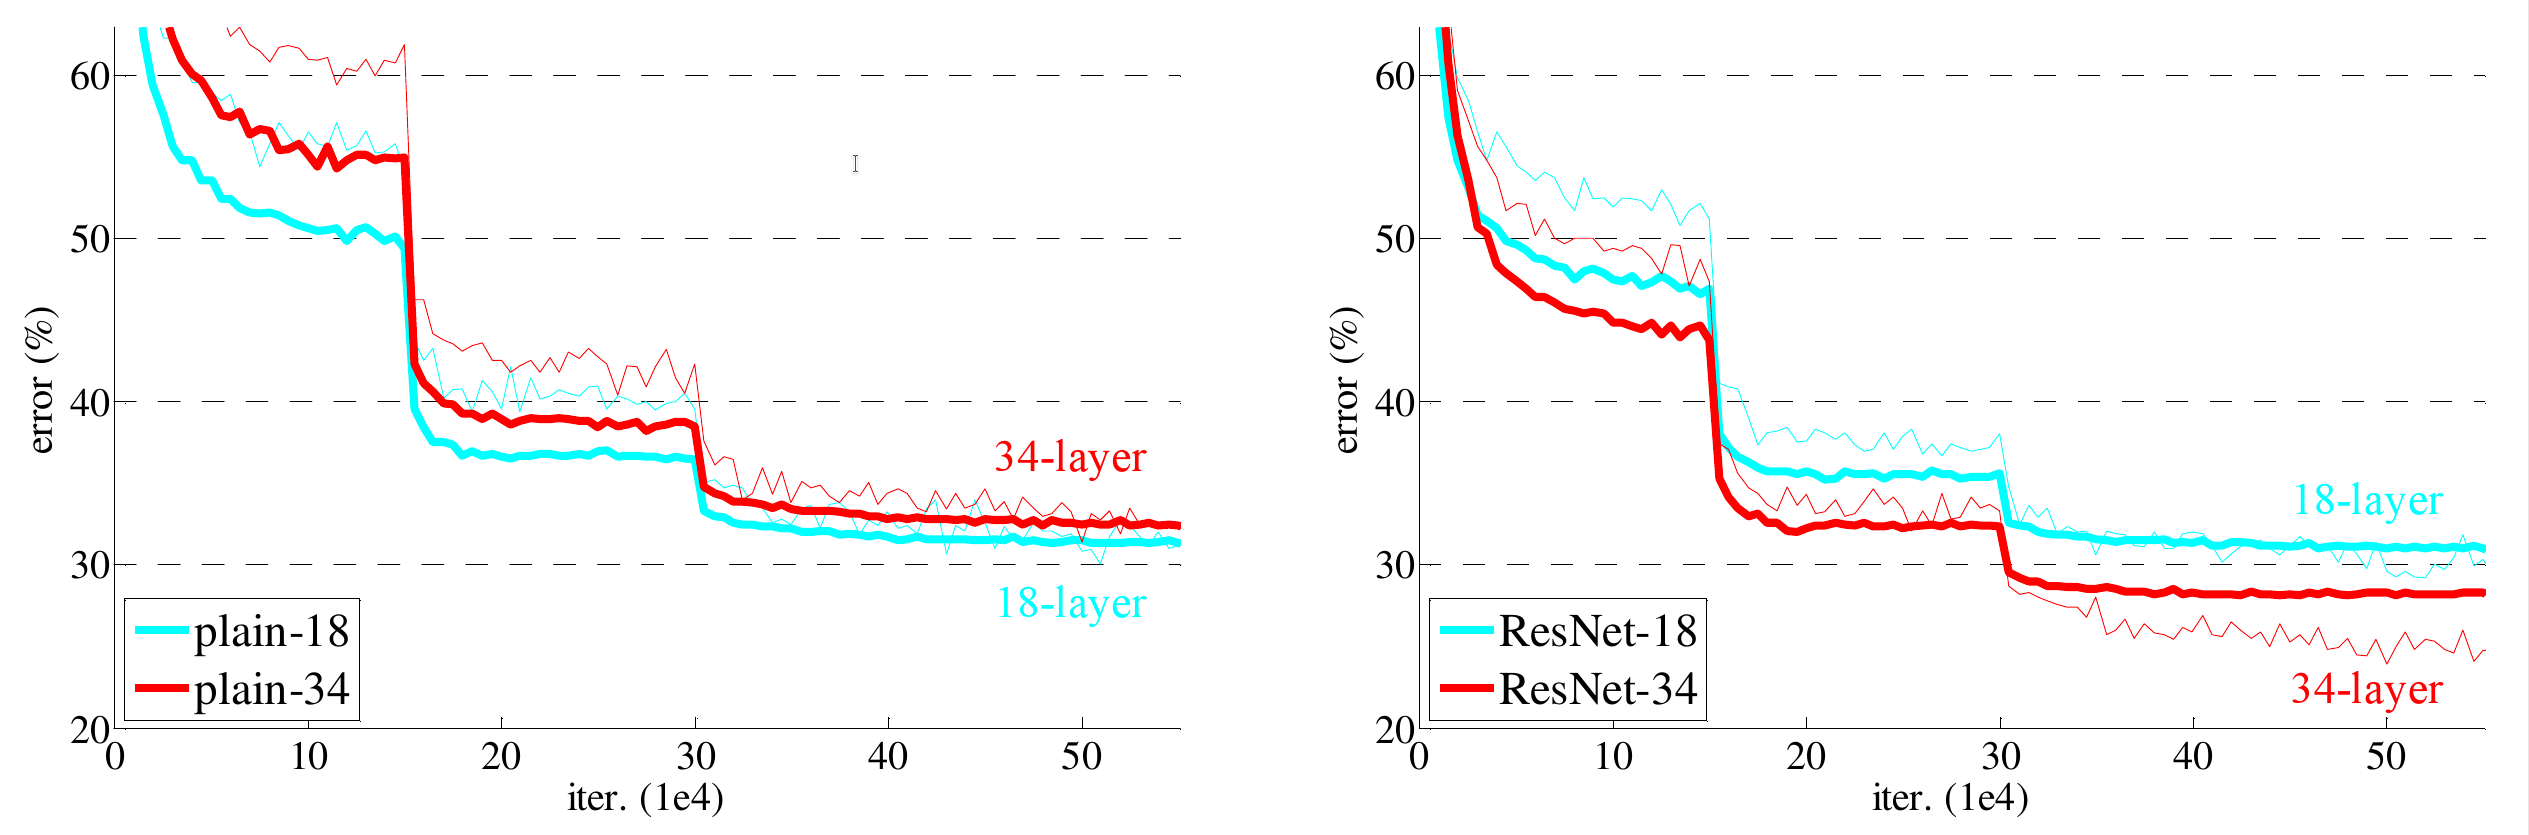
\includegraphics[scale=0.4]{figures/image_net_error_by_kaiming_he.png}
	}
	\caption{
		Training (thin) and validation errors (bold) for a 18- and 34-layer plain network (left) and ResNet (right).
		The plain 34 layer network shows worse results than the 18 layer equivalent, whereas the deeper ResNet performs better than the 18 layer one.
		This is not the case for the plain network.
		This figure originates from the paper "Deep Residual Learning for Image Recognition" by \citet{he16}. \copyright~2016 IEEE.}
	\label{fig:depth-performance-decline}
\end{figure}

%Yet in practice one can observe deteriorating performance after a certain depth has been reached.
%An example for this can be seen in \cref{fig:depth-performance-decline} on the left.
These facts indicate that deeper networks are more efficient and should generally perform better than shallow ones.
Nonetheless, the example in \cref{fig:depth-performance-decline} shows the opposite effect.
It seems that contemporary optimizers are not able to effectively learn the constructed, deeper solution presented above.
\citet{he16} conjecture that this is because it is hard to learn the identity mapping through non-linear layers and suggest that it is easier to learn the zero function instead.
This leads to their proposed network architecture: Residual Neural Networks.

The characteristic feature of ResNets is that they learn residual mappings instead of unreferenced mappings.
Let $f: \cX \rightarrow \cX$ be the function to be approximated by number of (non-linear) layers and $x \in \cX$.
\citet{he16} suggest that instead of learning $f$ directly, to learn the \emph{residual}; given by
\begin{equation}
	\begin{split}
		g: \cX \rightarrow \cX \\
		g(x) \coloneqq f(x) - x \ .
	\end{split}
\end{equation}
This is implemented by creating shortcut connections that skip one or more layers and add the input to the layers' output, resulting in $g(x) + x = f(x)$.
An illustration of a typical residual block is shown in \cref{fig:residual-block}.

\begin{figure}
	\centering
	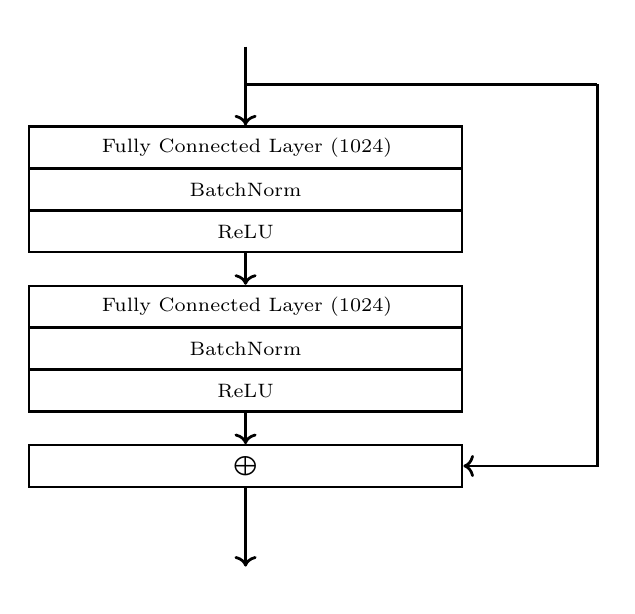
\begin{tikzpicture}
		[
		font=\scriptsize,
		block/.style ={rectangle, draw=black, thick, text width=15em, align=center, minimum height=1.5em}
		]
		\node[] (a) [block] {Fully Connected Layer (1024)};
		\node[below= -1.5\pgflinewidth of a] (a1) [block] {BatchNorm};
		\node[below= -1.5\pgflinewidth of a1] (b) [block] {ReLU};
		\node[below= 4mm of b] (c) [block] {Fully Connected Layer (1024)};
		\node[below= -1.5\pgflinewidth of c] (c1) [block] {BatchNorm};
		\node[below= -1.5\pgflinewidth of c1] (d) [block] {ReLU};
		\node[below= 4mm of d] (e) [block] {$\bigoplus$};
		\node[above=of a] (x) [] {};
		\draw[->, line width=1pt] (b.south) -- (c.north);
		\draw[->, line width=1pt] (d.south) -- (e.north);
		\draw[->, line width=1pt] (x) -- (a);
		\node[below=of e] (y) [] {};
		\draw[->, line width=1pt] (e) -- (y);
		\node[above=.4 of a] (z) [] {};
		\node[right=12em of z] (h) [] {};
		\draw[line width=1pt] (z.center) -- (h.center);
		\draw[->, bend right, line width=1pt] (h.center) |- (e.east);
	\end{tikzpicture}
	\caption{Typical residual block.
	$\bigoplus$ indicates the inputs of both arrows being summed.
	This particular design was used in \cite{drover18} for 3D Human Pose Estimation.
	Similar blocks are used in image classification and object detection, where the fully connected layers are usually replaced by convolutions.
	}
	\label{fig:residual-block}
\end{figure}

This residual network layout was able to circumvent the decrease in performance that came with an increased number of layers and even showed better results, as one would expect from a model with a greater number of parameters.
Nowadays, ResNets have become an essential part of network architectures and are used in virtually all areas of machine learning, including image classification and object detection \cite{he16,carion20}, semantic segmentation \cite{chen17}, 3D human pose estimation \cite{drover18} and natural language processing \cite{keskar19,conneau16,vaswani17}.

	
	\section{Mathematical Preliminaries}
\label{sec:preliminaries}

This section provides a brief introduction to the most important theories from which the concept of mechanical regression is derived in \cref{sec:mechanical-regression}.
Those involve some functional analysis, in particular Reproducing Kernel Hilbert Spaces, some notation for product spaces and specific loss functions.

\subsection{Reproducing Kernel Hilbert Spaces}

\section{Reproducing Kernel Hilbert Spaces}

\begin{definition}[RKHS]
	\label{def:rkhs}
	content...
\end{definition}

\begin{definition}[Kernel]
	\label{def:kernel}
\end{definition}

\begin{theorem}
	\label{theo:kernel-for-rkhs}
	For every RKHS $\mathfrak{H}$ there exists a unique associated Kernel $K$.
\end{theorem}
\begin{proof}[Idea of proof]
	content...
\end{proof}

Example: Gaussian/RBF-Kernel, Polynomial Kernel

\subsection{Features Space and Feature Maps}

\begin{equation}
	\label{eq:kernel-feature-map}
	K(x_1, x_2) = \psi^\T(x_1)\psi(x_2)
\end{equation}

\begin{theorem}
	\begin{equation}
		\left< \psi^\T(\cdot) \alpha, \psi^\T(\cdot) \beta\right>_\mathcal{H} = \left< \alpha, \beta\right>_\mathcal{F} \ .
	\end{equation}
\end{theorem}
\begin{corollary}
	\label{cor:feature-space-norm}
	\begin{equation}
		\norm{\psi^\T(\cdot)\alpha}_\mathcal{H}^2 = \norm{\alpha}_\mathcal{F}^2 \ .
	\end{equation}
\end{corollary}

\subsection{Product Space and Block Operator Notation}
Later on, it would be quite cumbersome to always treat the $X_i$ separately.
Hence we will now introduce block operator syntax which will enable us to write equations more concisely.
As in later parts we will almost exclusively rely on this notation, we first have to make sure that all used syntax is mathematically correct.
In the following we will define the product space of $\cY$, some useful notation and assure that all future calculations involving that new notation are mathematically sound.

Let $\cY^N \coloneqq \bigtimes_{i=1}^N \cY$ be the $N$-fold product space and $A, B \in \cY^N$.
Defining $\left < A, B \right >_{\cY^N} \coloneqq \sum_{i=1}^{N} \left <A_i, B_i \right >$ fulfills the properties of an inner product on $\cY^N$ and thus makes $\cY^N$ a Hilbert Space itself.


\begin{definition}[Block Operator Matrix]
	A \emph{Block Operator Matrix} $\mathbf{A}$ is an $(N \times N)$-Matrix with Elements in $\cL(Y, Y)$.
\end{definition}

\begin{definition}[$\cY^N$]
	content...
\end{definition}
Explain: We can express the corresponding inner product as matrix multiplication.

\begin{theorem}
	$(\cL(\cY^N, \cY^N), +, \circ)$ is a  ring.
\end{theorem}
\begin{proof}
	We conduct the proof by showing that $\cL(\cY^N, \cY^N) \cong \R^{nN \times nN}$.
\end{proof}

As a consequence of the proof, we get the following corollary.
\begin{corollary}
	\label{cor:matrix-ring-equivalence}
	$\cL(\cY^N, \cY^N) \cong \R^{nN \times nN}$.
\end{corollary}

\begin{corollary}
	\label{cor:matrix-vector-equivalence}
	Block-Operator Matrix times vector is isomorphic to standard matrix times vector.
\end{corollary}

\begin{figure}
	This will be an illustration of isomorphisms in the block operator matrix example.
	\caption{And this will be the supercool caption.}
	\label{fig:block-operator-example}
\end{figure}

\begin{example}
	Let $\cY = \R^n$.
	\Todo{Discard Example, make it lemma/theorem.
		Replace $\R$ by general field, as Hilbert Spaces are vector spaces,
		make first isomorphism monoid homomorphism, maybe even ring homomorphism.
		This means we can work with $\mathbf{K}$ just like a regular matrix.
		Check if $\mathbf{K}$ really is symmetric or not just hermitian.
		Also prove that there is an inverse under certain circumstances.}
	Then we have $\cL(\cY) \cong \R^{n\times n}$, which means applying a (bounded) linear operator to a $y \in \cY$ can be expressed as matrix-vector multiplication.
	We now claim that in this case $\cL(\cY^N) \cong \R^{nN \times nN}$ and that the computation of $\mathbf{A}\cdot \mathbf{y}$ can be expressed as a standard matrix-vector product.
	For the first part, let $\mathbf{A} \in \cL(\cY^N)$ and $\mathbf{y} \in \cY^N$. 
	Write $\mathbf{A} = (\mathbf{A}_{i, j})$ with $\mathbf{A}_{i,j} \in \cL(\cY)$. 
	We obtain the corresponding $(nN \times nN)$-matrix by first applying the canonical isomorphism $\cL(\cY) \cong \R^{n\times n}$ to each $\mathbf{A}_{i,j}$ and then "flattening" the result.
	For the second part, we first have to consider another isomorphism $\cY^N \cong \R^{nN}$ which is given by consecutively pasting the elements of $\cY^N$ into one vector of size $nN$.
	\cref{fig:block-operator-example} illustrates both isomorphisms.
	
	These new representations of $\mathbf{A}$ and $\mathbf{y}$ make it particularly easy to compute $\mathbf{A}\cdot \mathbf{y} = \mathbf{x}$:
	Simply map $\mathbf{A}$ to $A \in \R^{nN \times nN}$ and $\mathbf{y}$ to $y \in \R^{nN}$, calculate $A \cdot y = x$ as the standard matrix-vector product and map the resulting vector $x$ back to $\mathbf{x} \in\cY^N$.	
	\Todo{Image: Block Operator Matrix -> "flattened" Matrix}
\end{example}

With $K$ being the Kernel associated with the RKHS $\mathcal{H}$ and $A, B \in \cY^N$ we will write $\mathbf{K}(A, B)$ for the matrix with the entries $K(A_i, B_j)$ at position $(i, j)$.


\subsection{Optimal Recovery}
\label{sec:optimal-recovery}

\begin{theorem}[Representer Theorem]
	\label{theo:representer}
\end{theorem}

The optimal recovery loss is defined as
\begin{equation}
	\label{eq:optimal-recovery-loss}
	l(X, Y) \coloneqq \min\{\norm{f}_\mathcal{H}^2 ~|~ f\in \mathcal{H} \text{~and~} f(X) = Y\}
\end{equation}

By \cref{theo:representer}, the $f \in \mathcal{H}$ which minimizes \cref{eq:optimal-recovery-loss} admits a representation as 
\begin{equation}
	\label{eq:optimal-recovery-f}
	f(x) = \sum_{i=1}^N K(x, X_i) Z_i \ ,
\end{equation}
where the $Z_i$ are the solutions to the following linear system ($1 \leq j \leq N$):
\begin{equation}
	\sum_{i=1}^{N} K(X_j, X_i) Z_i = Y_j
\end{equation}
For better readability we translate this expression into block operator notation:
Introduce the block operator matrix $\mathbf{K}(X, X)$ with entries $K(X_i, X_j)$ and $Z = (Z_i)_{i \in [N]} \in \cY^N$.
Using block operator notation, we can write the linear system more concisely as $\mathbf{K}(X, X) \cdot Z = Y$.
Assuming the kernel $K$ is non-degenerate and the $X_i$ are pairwise distinct, we can, by \Todo{ref!}Lemma ??, find an inverse of $\mathbf{K}(X, X)$ and write $Z = \mathbf{K}(X, X)^{-1} \cdot Y$.

Let $x \in X$ and $\mathbf{K}(x, X)$ be the vector with elements $K(x, X_i)$.
Using this notation, we can rewrite \cref{eq:optimal-recovery-f} as
\begin{equation}
	f(x) = \mathbf{K}(x, X) \cdot \mathbf{K}(X, X) \cdot Y \ .
\end{equation}
The value of the loss function is the $\mathcal{H}$-norm of this $f$.
As $\mathcal{H}$ is a Hilbert Space, we can compute it using the scalar product:
\begin{align}
	\norm{f}_\mathcal{H}^2 &= \left< f, f\right>_\mathcal{H}\\
	&= \left< \sum_{i=1}^N K(x, X_i) Z_i, \sum_{i=1}^N K(x, X_j) Z_j \right>_\mathcal{H}\\
	&= \sum_{i=1}^N \sum_{j=1}^N \left< K(x, X_i) Z_i, K(x, X_j) Z_j \right>_\mathcal{H}\\
	&= \sum_{i=1}^N \sum_{j=1}^N \left< Z_i, K(X_i, X_j) Z_j \right>_\cY\\
	&= \left< Z, \mathbf{K}(X, X) \cdot Z\right >_{\cY^N}\\
	&= Z^\T \cdot \mathbf{K}(X, X) \cdot Z \\
	&= (\mathbf{K}(X, X)^{-1} \cdot Y)^\T \cdot \mathbf{K}(X, X) \cdot \mathbf{K}(X, X)^{-1} \cdot Y\\
	&= Y^\T \cdot (\mathbf{K}(X, X)^{-1})^\T \cdot Y\\
	&=  Y^\T \cdot \mathbf{K}(X, X)^{-1} \cdot Y \ .
\end{align}
In the fourth line we used the reproducing property and in the second to last line the fact $\mathbf{K}$ that $K$ is Hermitian, that is, $K(x, y)^\T = K(y, x)$.
All in all, this leaves us with an appealing and compact form for the optimal recovery loss:
\begin{equation}
	l(X, Y) = Y^\T \mathbf{K}(X, X)^{-1} Y \ .
\end{equation}
\subsection{Ridge Regression}

\begin{equation}
	\label{eq:ridge-regression-loss}
	l(X, Y) \coloneqq \inf_{f \in \mathcal{H}} \lambda \norm{f}_\mathcal{H}^2 
	+ l_\cY (f(X), Y)
\end{equation}

\begin{equation}
	\label{eq:ridge-regression-f}
	f(x) = \mathbf{K}(x, X)^\T \left(\mathbf{K}(x, X) + \lambda I\right)^{-1}Y \ .
\end{equation}
Ridge regression can be seen as a Tikhonov-regularized variant of optimal recovery.

%\subsection{Feature Space and Feature Maps}
%
%Next, we define feature spaces and feature maps.
They are of special interest in machine learning and are especially relevant for Support Vector Machines (SVMs) \cite{steinwart08}, where they enable learning non-linear decision functions.
\citet{steinwart08} give an extended introduction to kernels, feature maps and feature space for the scalar case.
Here, we will follow \cite{owhadi20} and define these terms for the more general case of operator-valued kernels.
We will mainly present results which are relevant for later sections.

\begin{definition}
	\label{def:feature-map-space}
	A Hilbert space $\cF$ and a function $\psi: \cX \rightarrow L(\cY, \cF)$ are \emph{feature space} and \emph{feature map} for the Kernel $K$ if for all $x_1, x_2 \in \cX, y_1, y_2 \in \cY$:
	\begin{equation}
		\left< y_1, K(x_1, x_2) y_2\right>_\cY = \left< \psi(x_1) y_1, \psi(x_2) y_2\right>_\cF \ .
	\end{equation}
\end{definition}

The Kernel $K$ does in itself induce a feature map and space.
The following example is an extension of \cite[Lemma~4.19]{steinwart08}, where the canonical feature map of $K$ is defined for the scalar case.
\begin{example}[Canonical feature map for operator-valued kernel]
	Define $\psi(x) \coloneqq \left(y \rightarrow K(\cdot, x)y\right)$.
	Then $\psi$ is a function $\cX \rightarrow L(\cY,\cH)$ because $K(\cdot, x) y \in \cH$ by definition.
	Furthermore we have for all $x_1, x_2 \in \cX$ and $y_1, y_2 \in \cY$:
	\begin{align}
		\left<\psi(x_1) y_1, \psi(x_2)y_2 \right>_\cH &= 
		\left< K(\cdot, x_1) y_1, K(\cdot, x_2) y_2\right>_\cH\\
		& = \left< K(x_2, x_1) y_1, y_2 \right>_\cY \\
		& = \left< y_1, K(x_2, x_1)^\T y_2 \right>_\cY\\
		& = \left< y_1, K(x_1, x_2) y_2\right>_\cY \ .		
	\end{align}
	This makes $\psi$ a feature map and $\cH$ a feature space for $K$. \qed
\end{example}

Let $\psi^\T: \cX \rightarrow L(\cF, \cY)$ be the adjoint of $\psi$ in the sense that for all $x \in \cX, y\in \cY, \alpha \in \cF$
\begin{equation}
 \left< \psi(x)y, \alpha\right>_\cF = \left<y, \psi^\T(x) \alpha \right>_\cY \ .
\end{equation}
With the adjoint we can derive a concise equation for the kernel $K$:
\begin{align}
	\left< y_1, K(x_1, x_2) y_2\right>_\cY = \left< \psi(x_1) y_1, \psi(x_2) y_2\right>_\cF = \left<y_1, \psi^\T(x_1)\psi(x_2) y_2\right>_\cY \ .
\end{align}
As this holds true for all $x_1, x_2 \in \cX, y_1, y_2 \in \cY$, we conclude
\begin{equation}
\label{eq:kernel-feature-map}
K(x_1, x_2) = \psi^\T(x_1) \psi(x_2) \ .
\end{equation}
Note that composing $\psi^T(x) \circ \psi(x)$ does indeed result in a function $\cY \rightarrow \cY$, which matches the target type of $K$.

Using $\psi^\T$ and $\alpha \in \cF$, we can also define functions $\cX \rightarrow \cY$:
\begin{align}
		\psi^\T\alpha: ~&\cX \rightarrow \cY \\
		(\psi^\T\alpha)(x) &\coloneqq \psi^\T(x)\alpha \ .
\end{align}
Without loss of generality we can restrict $\cF$ to the image of the function
\begin{align}
	\varphi: ~&\cX \times \cY \rightarrow \cF\\
	\varphi(x, y) &\coloneqq \psi(x)y\ .
\end{align}
We will not detail why this is possible.
\Todo{Maybe it is straightforward to see that cF is still Banach in this case.It is clear that the inner product still works.}
It especially requires $\mathrm{im}(\varphi)$ to be a Hilbert space.
The intuition behind this ...
\Todo{Intuition: Move from X to some weird high dimensional space which allows learning non linearities.
But it doesnt really matter what this feature space cF looks like as we dont have to care about it.
Therefore we can restrict F to whatever we want - as long as it makes sense.}
Restricting $\cF$ like this has the advantage that $\cH$ is then equal to the closure of the span of $\{\psi^\T\alpha\ |\ \alpha \in \cF\}$.
From this result we obtain the following theorem.
\begin{theorem}
	\label{theo:f-h-correspondence-equation}
	If $\cF = \mathrm{im}(\varphi)$ it holds true that for all $\alpha, \beta \in \cF$ 
	\begin{equation}
		\left< \psi^\T(\cdot) \alpha, \psi^\T(\cdot) \beta\right>_\cH = \left< \alpha, \beta\right>_\cF \ .
	\end{equation}
\end{theorem}
\begin{proof}
	Using the reproducing property we first have for $\alpha \in \cF, x \in \cX$ and $y \in \cY$ that
	\begin{align}
		\left<\psi^\T(\cdot) \alpha, \psi^T(\cdot)\psi(x)y\right>_\cH
		&= \left<\psi^\T(\cdot) \alpha, K(\cdot, x) y \right>_\cH \\
		&= \left<\psi^\T(x)\alpha, y\right>_\cY\\
		&= \left<\alpha, \psi(x)y\right>_\cF \ .
	\end{align}
	Let $\beta \in \cF$.
	Then $\beta \in \mathrm{im}(\varphi)$, implying there exist $x \in \cX, y \in \cY$ such that $\varphi(x, y) = \beta$.
	Substituting $\psi(x)y = \beta$ in the first and last line of the equation above proves the claim.
\end{proof}
We conclude this section with the following result, which is an immediate consequence of \cref{theo:f-h-correspondence-equation}.
\begin{corollary}
	\label{cor:feature-space-norm}
	\begin{equation}
		\norm{\psi^\T(\cdot)\alpha}_\cH^2 = \norm{\alpha}_\cF^2 \ .
	\end{equation}
\end{corollary}


\subsection{Product Space and Block Operator Notation}
\label{sec:block-operator-notation}

This section gives a brief introduction to the block operator notation used in later sections.
It allows simpler and more concise notation for vectors like $X \in \cX^N$ and $Y \in \cY^N$ for what would otherwise require statements on an vector entry basis.
Although most of the time the notation will seem intuitive, we still have to ensure that all transformations involving it are mathematically sound.

Block operator matrices are defined on the $N$-fold product space of $\cY$.
As a short reminder, the $N$-fold product space of $\cY$ is defined as $\cY^N \coloneqq \bigtimes_{i=1}^N \cY$.
The inner product on $\cY$ can be extended to $\cY^N$ in a natural way:
Let $A, B \in \cY^N$.
Then $\left < A, B \right >_{\cY^N} \coloneqq \sum_{i=1}^{N} \left <A_i, B_i \right >$ fulfills the properties of an inner product on $\cY^N$ and thus makes $\cY^N$ a Hilbert space.

\begin{definition}[Block Operator Matrix]
	A \emph{Block Operator Matrix} $\mathbf{A}$ is an $(N \times N)$-Matrix with Elements in $L(\cY, \cY)$.
\end{definition}
\Todo{By definition of the product space L(YN, YN) is isomorphic to L(Y, Y)NxN}
Although the definition of block operator matrices does not involve the product space, they are closely connected, which can be seen in the following lemma.
\begin{lemma}
  $L(\cY, \cY)^{N \times N} \cong L(\cY^N, \cY^N)$.
\end{lemma}
The proof is quite intuitive and will not be conducted here.

For $\mathbf{A} \in L(Y, Y)^{N\times N}$ and $U \in \cY^N$ we can define a function
\begin{align}
	\sigma:~&L(Y, Y)^{N\times N} \times \cY^N \rightarrow \cY^N \\
	\sigma(\mathbf{A}, U) & = V \coloneqq \mathbf{A} \cdot U\ \text{, where $V$ is defined as} \\
	V_{i, j} &\coloneqq \sum_{k = 1}^N \mathbf{A}_{i,k} \cdot U_{k, j} \\
\end{align}
This is similar to the standard matrix-vector product known from linear algebra.
The only difference is that instead of multiplying elements of a field, we here apply the operator $\mathbf{A}_{i, j}$ to element $U_{k, j} \in \cY$.
It already seems like block operator matrices can be treated as regular matrices, but this has not been proven yet.
We will show two important properties: That block operator matrices form a ring and that we can treat $\sigma$ like the standard matrix-vector product.

\begin{theorem}
	\label{theo:product-space-ring}
	$(L(\cY, \cY)^{N\times N}, +, \circ)$ is a  ring.
\end{theorem}
\begin{proof}
	We conduct the proof by showing that $\cL(\cY^N, \cY^N) \cong \dK^{nN \times nN}$, where $\dK = \R$ or $\dK = \mathbb{C}$ is the underlying field.
	Let $\mathbf{A} \in L(\cY^N, \cY^N)$ $n \coloneqq \mathrm{dim}(\cY) < \infty$ (we required $\cY$ to be finite).
	First, we have $\cL(\cY) \stackrel{\phi}{\cong}\R^{n\times n}$ by mapping an operator to its transformation matrix with respect to a fixed choice of basis.
	Thus we can regard $\mathbf{A}$ as a big $(N \times N)$ matrix of $(n \times n)$ matrices.
	Actually, $\phi$ induces an isomorphism $L(\cY^N, \cY^N) \cong \left(\dK^{nxn}\right)^{N \times N}$.
	Now, the idea is to define $\xi:\left(\dK^{nxn}\right)^{N \times N} \rightarrow \dK^{nN \times nN}$ as the function that "flattens" this matrix.
	This is visualized in \cref{fig:block-operator-example} and should suffice as a definition.
	One can easily check that $\xi \circ \phi$ is the desired isomorphism.
\end{proof}

\begin{figure}
	This will be an illustration of isomorphisms in the block operator matrix example.
	\caption{And this will be the supercool caption.}
	\label{fig:block-operator-example}
\end{figure}

As a consequence of the proof, we get the following corollary.
\begin{corollary}
	\label{cor:matrix-ring-equivalence}
	If $\cY$ is a real Hilbert space, $\cL(\cY, \cY) \cong \R^{nN \times nN}$.
\end{corollary}
Similarly, we get an isomorphism $\cY^N \cong \R^nN$.
These new representations of $\mathbf{A}$ and $U$ make it particularly easy to compute $\sigma$:
Simply map $\mathbf{A}$ to $A \in \R^{nN \times nN}$ and $\mathbf{y}$ to $y \in \R^{nN}$, calculate $A \cdot y = x$ as the standard matrix-vector product and map the resulting vector $x$ back to $\mathbf{x} \in\cY^N$.
This is summed up in the following diagram

\begin{corollary}
	\label{cor:matrix-vector-equivalence}
	\begin{equation}
		\begin{tikzcd}
		 	L(\cY^N, \cY^N) \arrow{r}{\delta_U} \arrow[swap, leftrightarrow]{d}{\cong} & \cY^N \arrow[leftrightarrow]{d}{\cong} \\%
			\R^{nN \times nN} \arrow{r}{\partial_V}& \R^{nN}
		\end{tikzcd}
	\end{equation}
\end{corollary}

\Todo{These facts make implementation easier, as we will see in section ?}

\subsection{Special Loss Functions}

In the following we will explore two special loss functions that will be relevant later on.
We assume $K$ to be a non-degenerate kernel associated to the RKHS $\cH$.

\subsubsection{Optimal Recovery}
\label{sec:optimal-recovery}

The optimal recovery loss is defined as
\begin{equation}
\label{eq:optimal-recovery-loss}
l(X, Y) \coloneqq \min\{\norm{f}_\cH^2 ~|~ f\in \mathcal{H} \text{~and~} f(X) = Y\}
\end{equation}
In the setting of the supervised learning problem, this loss aims to find the $f \in \cH$ with the smallest $\cH$-norm that still satisfies $f(X) = Y$ in order to approximate the target function $f^\dagger$.

As $\cH$ is an RKHS, we can derive a closed-form solution for $l(X, Y)$ and also for its minimizer $f$.
For that, we want to apply \cite[Theorem 3.1]{micchelli05}.
It requires the evaluation functionals $\{\delta_{X_i}: \cH \rightarrow \cY \ |\ \delta_{X_i}(f) = f(X_i), i \in [N]\}$ to be linearly independent.
By \cite[Lemma 3.1]{micchelli05} this is equivalent to the statement that for all $d_i \in \cY, i \in [N]$ there exist unique $c_i \in \cY, i \in [N]$ such that
\begin{equation}
	\sum_{k=1}^N K(X_i, X_k) c_k = d_k \ ,\ i \in [N] \ .
\end{equation}
We already know $X_i$ are pairwise distinct and $K$ is non-degenerate.
Applying \cref{lem:kernel-non-singular} gives that the matrix with entries $K(X_i, X_j)$ is non-singular, which implies the existence of such unique $c_k$.

This means we can now apply \cite[Theorem 3.1]{micchelli05} which states that the minimizer $f$ admits a representation as 
\begin{equation}
	\label{eq:optimal-recovery-f}
	f(x) = \sum_{i=1}^N K(x, X_i) Z_i \ ,
\end{equation}
where the $Z_i$ are the solutions to the following linear system:
\begin{equation}
	\sum_{i=1}^{N} K(X_j, X_i) Z_i = Y_j \ ,\ j \in [N] \ .
\end{equation}

For better readability we translate this expression into block operator notation:
Let $\mathbf{K}(X, X) \in L(\cY, \cY)^{N\times N}$ be the block operator matrix with entries $K(X_i, X_j)$ at position $(i, j)$ and $Z = (Z_i)_{i \in [N]} \in \cY^N$.
Then we can write the linear system more concisely as 
\begin{equation}
	\mathbf{K}(X, X) \cdot Z = Y \ .
\end{equation}
Because of the non-singularity of $\mathbf{K}(X, X)$ and the ring isomorphism in \cref{cor:matrix-ring-equivalence} we can find an inverse to $\mathbf{K}(X, X)$ and write $Z = \mathbf{K}(X, X)^{-1} \cdot Y$.

Now for $x \in X$, let $\mathbf{K}(x, X)$ be the vector with elements $K(x, X_i)$.
Using this notation, we can rewrite \cref{eq:optimal-recovery-f} in a concise way as
\begin{equation}
	f(x) = \mathbf{K}(x, X) \cdot \mathbf{K}(X, X) \cdot Y \ .
\end{equation}

With this representation for the optimal $f$ it easy to derive a closed-form expression for the value of the loss, which is just the squared $\mathcal{H}$-norm of the minimizer $f$.
We get
\begin{align}
	\norm{f}_\mathcal{H}^2 &= \left< f, f\right>_\mathcal{H}\\
	&= \left< \sum_{i=1}^N K(x, X_i) Z_i, \sum_{j=1}^N K(x, X_j) Z_j \right>_\mathcal{H}\\
	&= \sum_{i=1}^N \sum_{j=1}^N \left< K(x, X_i) Z_i, K(x, X_j) Z_j \right>_\mathcal{H}\\
	&= \sum_{i=1}^N \sum_{j=1}^N \left< K(X_j, X_i)Z_i, Z_j \right>_\cY\\
	&= \sum_{i=1}^N \sum_{j=1}^N \left< Z_i, K(X_j, X_i)^\T Z_j \right>_\cY\\
	&= \sum_{i=1}^N \sum_{j=1}^N \left< Z_i, K(X_i, X_j) Z_j \right>_\cY\\
	&= \left< Z, \mathbf{K}(X, X) \cdot Z\right >_{\cY^N}\\
	&= \left< \mathbf{K}(X, X)^{-1} \cdot Y, \mathbf{K}(X, X) \cdot \mathbf{K}(X, X)^{-1} \cdot Y\right >_{\cY^N} \\
	&= \left< \mathbf{K}(X, X)^{-1} \cdot Y,  Y\right >_{\cY^N}\\
	&= Y^\T \cdot (\mathbf{K}(X, X)^{-1})^\T \cdot Y\\
	&=  Y^\T \cdot \mathbf{K}(X, X)^{-1} \cdot Y \ .
\end{align}
In the fourth line we used the reproducing property and in the second to last line the fact that $K$ is Hermitian, which implies that $\mathbf{K}(X, X)$ is too.
All in all, this leaves us with an appealing and compact form for the optimal recovery loss:
\begin{equation}
	\label{eq:optimal-recovery-loss-closed-form}
	l(X, Y) = Y^\T \mathbf{K}(X, X)^{-1} Y \ .
\end{equation}

\subsubsection{Ridge Regression}

Another class of loss functions are the ridge regression losses, which are also known as as Tikhonov regularization.
They are also widely used in deep learning \cite{goodfellow16}.
In general, the ridge regression loss is defined as
\begin{equation}
	\label{eq:ridge-regression-loss}
	l(X, Y) \coloneqq \inf_{f \in \mathcal{H}} \lambda \norm{f}_\mathcal{H}^2 
	+ l_\cY (f(X), Y) \ ,
\end{equation}
where $l_\cY: \cY^N \times \cY^N \rightarrow \R$ is an arbitrary positive loss function and $\lambda > 0$ a balancing parameter.

For certain losses $l_\cY$, closed-form expressions can be derived similar to those for the optimal recovery loss.
As an example, we will take a look at the case where $l_\cY$ is the empirical squared error, given by
\begin{equation}
	l_\cY(Y_1, Y_2) = \sum_{k=1}^{N} \norm{Y_{1, k} - Y_{2, k}}_\cY^2 \ .
\end{equation}
We will not show the whole derivation of the expressions, but take a look at the results.
For the squared error, the ridge regression optimizer $f$ can be represented as
\begin{equation}
	\label{eq:ridge-regression-f}
	f(x) = \mathbf{K}(x, X)^\T \left(\mathbf{K}(x, X) + \lambda I\right)^{-1}Y \ .
\end{equation}
Let $\mathbbm{1}_N$ be the $(N\times N)$ identity matrix.
Then the value of the loss for that minimizer is given as
\begin{equation}
	\label{eq:ridge-regression-loss-se-closed-form}
	l(X, Y) = \lambda Y^\T (\mathbf{K}(X, X) + \lambda \mathbbm{1}_N)^{-1} Y \ .
\end{equation}
%
%\subsection{Equivalence of Optimization Problems}
%\Todo[inline]{Probably remove this section.}
%\begin{definition}
%	\label{def:equivalent-problems}
%	Let $f: X \rightarrow \R$ and $g: Y \rightarrow \R$ be the target functions of two optimization problems $A$ and $B$.
%	Then $A$ and $B$ are \emph{equivalent} if there exists a bijection $\varphi: X \rightarrow Y$ such that
%	\begin{equation}
%		x \in X \text{~is optimal for A~} \Leftrightarrow \phi(x) \in Y \text{~is optimal for A~}\ .
%	\end{equation}
%\end{definition}
	
	\section{Mechanical Regression}

\Todo{Include figure of typical ResNet Layout}
Artificial Neural Networks are a popular method to solve the Supervised Learning problem described in Section X.
Especially Residual Neural Networks have shown great success in enabling very deep models.
As described earlier, RNNs usually consist of several Residual Blocks followed by dense mapping to the target space $Y$.
This section essentially follows Chapter 3 in \cite{owhadi20} and aims to provide a profound and comprehensive explanation of Mechanical Regression and how it can be interpreted as the continuous limit of ANNs, concretely RNNs.



We will now take a similar approach and try to approximate the target function $f^\dagger$ by a function
\begin{equation}
	f^\ast \coloneqq f \circ \Phi_L \ ,
\end{equation}
where 
\begin{equation}
	\Phi_L \coloneqq \phi_L \circ \phi_{L-1} \circ \ldots \circ \phi_1
\end{equation} 
is the composition of $L$ Residual Blocks, that is, functions $\phi_k = I + v_k$.
Here, the $v_k$ are functions mapping the input space $\cX$ onto itself and $I$ is the identity operator.
Thus, we can regard $\Phi_L$ as a large deformation of $\cX$.
$f: \cX \to \cY$ is a function mapping the deformed space to the target space $\cY$.

By default, the $v_k$ and $f$ can be arbitrary functions.
\Todo{ref: chapter on regularization in Deep Learning? At least explain further!}
Thus, as common in Machine Learning, in order to avoid overfitting the functions to the data, we penalize $v_k$s and $f$s with large norms.
For that, we introduce two RKHSs:
$\mathcal{V} \subseteq \{\cX \rightarrow \cX\}$ and $\mathcal{H} \subseteq \{\cX \rightarrow \cY\}$. 
By \cref{theo:kernel-for-rkhs} there is a Kernel associated with each RKHS.
Let $\Gamma$ be the Kernel associated with $\mathcal{V}$ and $K$ that of $\mathcal{H}$.
We then can identify $f$ and the $v_k$ as solutions to the following problem:
\begin{problem}
	\label{prob:min-v-f}
	\begin{cases}
		\text{Minimize~} & \nu \cdot \frac{L}{2} \sum_{k=1}^{L} \norm{v_k}_\mathcal{V}^2
		+ \lambda \norm{f}_\mathcal{H}^2 
		+ l((f \circ \Phi_L)(X), Y) \\
		\text{such that~} & v_1, \ldots, v_L \in \mathcal{V}, f \in \mathcal{H} \ .
	\end{cases}
\end{problem}
Here, $\nu$ and $\lambda$ are strictly positive balancing parameters.
$l$ is a (positive) loss measuring the similarity of the predicted outputs, that is, the image of $X$ under $f \circ \Phi_L$.

Utilizing the Ridge Regression Loss $l_R$ (\cref{eq:ridge-regression-loss}), we can rewrite the above minimization problem as
\begin{problem}
	\begin{cases}
		\text{Minimize~} & \nu \cdot \frac{L}{2} \sum_{k=1}^{L} \norm{v_k}_\mathcal{V}^2
		+ l_R(\Phi_L(X), Y) \\
		\text{such that~} & v_1, \ldots, v_L \in \mathcal{V}\ .
	\end{cases}
\end{problem}
By "hiding" the regularity of $f$ in the loss we can for now focus on the functions $v_k$.
For our calculations we will therefore only assume that $l: \cX^N \times \cY^N \rightarrow$ is a positive, continuous loss function.
If desired we can later balance the $v_k$ with the regularity of $f$ by choosing the loss appropriately.

Our main goal will now be to show that the minimization problem in \cref{prob:min-v-f} can in fact be considered as a discrete solver of a mechanical system.
In order to do that, we first reformulate the problem by introducing additional variables $q_{i,j}$ with $2 \leq i \leq L+1$, $1 \leq j \leq N$:
\begin{align}
	q_{1, j} &\coloneqq X_j \, \\
	q_{i, j} &\coloneqq (\phi_{i-1} \circ \ldots \circ \phi_1) (X_j) \ .
\end{align}
Write $q_i$ for the vector with entries $q_{i,j}$ and hence we get $q_1 = X$ and $q_i = \phi_i(q_{i-1})$.
Regard the following minimization problem:
\begin{problem}
	\label{prob:min-q}
	\begin{cases}
		\text{Minimize~} & \nu \cdot \frac{1}{2} \sum_{k=1}^{L} \frac{(q_{k+1} - q_k)^\mathrm{T}}{\Delta t} \mathbf{\Gamma}(q_k, q_k)^{-1} \left(\frac{q_{k+1} - q_k}{\Delta t}\right) \Delta t+ l(q_{L+1}, Y) \\
		\text{such that~} & q_1 = X \text{~and~} q_2, \ldots, q_{L+1} \in \cX^N \ .
	\end{cases}
\end{problem}
We will now prove that \cref{prob:min-q} is in fact equivalent to \cref{prob:min-v-f} and, assuming we know the solution to the latter problem, provides us with an explicit solution for the $v_k$s.

\begin{theorem}
	$v_1, \ldots, v_L \in \mathcal{V}$ minimize \cref{prob:min-v-f} 
	$\Leftrightarrow$
	$q_1, \ldots, q_{L+1} \in \cX^N$ minimize \cref{prob:min-q} and
	$v_k(x) = \mathbf{\Gamma}(x, q_k)^\mathrm{T}\mathbf{\Gamma}(q_k, q_k)^{-1} (q_{k+1} - q_k)$.
\end{theorem}
\begin{proof}
	Using the above defined $q_k$ we have $v_k(q_k) = q_{k+1} - q_k$ for all $k \in [L]$.
	With that we can rewrite \cref{prob:min-v-f} as
	\begin{problem}
		\label{prob:min-q-v}
		\begin{cases}
			\text{Minimize~} & \nu \cdot \frac{L}{2} \sum_{k=1}^{L} \norm{v_k}_\mathcal{V}^2
			+ l(q_{L+1}, Y) \\
			\text{such that~} & v_1, \ldots, v_L \in \mathcal{V},\ \forall k \in [L]: v_k(q_k) = q_{k+1} - q_k, \\
			& q_1 = X \text{~and~} q_2, \ldots, q_{L+1} \in \cX^N \ .
		\end{cases}
	\end{problem}
	Here we just added the $q_k$ as additional variables but then bound them to certain values, concretely $q_{k+1} = q_k + v_k(q_k) = \phi_k(q_k)$, with $q_1 = X$.
	Recursively we get $q_{L+1} = \Phi_L(X)$ which means the target function remains the same as in \cref{prob:min-v-f}.
	Note that even though we seemingly added restraints to the domains of the $v_k$ they are still the same: We just have to choose $q_{k+1}$ accordingly (which we can, as it is unconstrained).
	
	We will now derive closed form expressions for the $v_k$ as a function of the $q_k$.
	For that, let $q_k \in \cX^N$, $2 \leq k \leq N$ be arbitrary but fixed .
	This means $l(q^{L+1}, Y)$ is constant and $v_k \in V_{k, q} \coloneqq \{v \in \mathcal{V}~|~ v_k(q_k) = q_{k+1} - q_k\}$.
%	These sets remain convex: Let $\lambda \in [0, 1]$ and $v_{k, 1}, v_{k, 2} \in V_{k, q}$, then we get
%	\begin{align}
%		(\lambda v_{k, 1} + (1 - \lambda) v_{k, 2})(q_k) &= (\lambda v_{k, 1})(q_k) + ((1 - \lambda) v_{k, 2})(q_k)\\
%		&=\lambda(q_{k+1} - q_k) + (1 - \lambda)(q_{k+1} - q_k)\\
%		&= q_{k+1} - q_k \ .
%	\end{align}
	We end up with a problem of the following form:
	\begin{problem}
		\begin{cases}
			\text{Minimize} &\sum_{i=1}^n f_i(x_i)\\
			\text{such that} & \forall i \in [n]: x_i \in A_i \ ,
		\end{cases}
	\end{problem}
	with bounded $f_i: A_i \rightarrow \R$.
	One can easily verify that minimization problems of this type have a global minimum at $x_i^\ast = \argmin\{f_i(x_i)~|~ x_i \in A_i\}$, the boundedness ensuring that at least one such minimum exists.

	Thus, we have to find the minima of $\min\{\norm{v_k}_\mathcal{V}^2~|~ v_k \in \mathcal{V}, v_k(q_k) = q_{k+1} - q_k\} = l_{\text{OR}}(q_k, q_{k+1} - q_k)$, $l_{\text{OR}}$ being the optimal recovery loss from \cref{sec:optimal-recovery}.
	From that section we conveniently get the following representations for the minimal $v_k$ and the target value:
	\begin{align}
		v_k & = \mathbf{\Gamma}(x, q_k)^\mathrm{T}\mathbf{\Gamma}(q_k, q_k)^{-1} (q_{k+1} - q_k)\\
		\norm{v_k}_\mathcal{H}^2 &= (q_{k+1} - q_k)^\mathrm{T} \mathbf{\Gamma}(q_k, q_k)^{-1} (q_{k+1} - q_k)
	\end{align}
	Here, $\mathbf{\Gamma}$ is the block operator matrix with entries $\Gamma(q_{k,i}, q_{k, j})$ and $\mathbf{\Gamma}(x, q_k)$ the vector $(\Gamma(x, q_{k, i}))_{i \in [N]}$.
	++
	Having now computed optimal $v_k$ -- or rather their squared $\mathcal{H}$-norms -- as a function of $q_2, \ldots, q_{L+1}$ we can reformulate \cref{prob:min-q-v} without the $v_k$ as variables.
	Define $\Delta t \coloneqq \frac{1}{L}$.
	We get:
	\begin{problem}
		\begin{cases}
			\text{Minimize~} & \nu \cdot \frac{1}{2} \sum_{k=1}^{L}  
			\left(\frac{q_{k+1} - q_k}{\Delta t}\right)^\mathrm{T} \mathbf{\Gamma}(q_k, q_k)
			\left(\frac{q_{k+1} - q_k}{\Delta t}\right) \cdot \Delta t
			+ l(q_{L+1}, Y) \\
			\text{such that~} & q_1 = X \text{~and~} q_2, \ldots, q_{L+1} \in \cX^N \ .
		\end{cases}
	\end{problem}
	As all steps and transformations hold true in both ways, this concludes the proof.
\end{proof}

\subsection{Least Action Principle}

Take a closer look at the first term of the objective function in \cref{prob:min-q} (the parameter $\nu$ has been deliberately omitted here):
\begin{equation}
	\label{eq:discrete-lagrangian}
	\frac{1}{2} \sum_{k=1}^{L} \left(\frac{q_{k+1} - q_k}{\Delta t}\right)^\mathrm{T} \mathbf{\Gamma}(q_k, q_k)^{-1} \frac{q_{k+1} - q_k}{\Delta t} \Delta t \ .
\end{equation}
With some imagination this very much looks like an approximation of the integral of some continuous function with a step function using $L$ intervals of width $\Delta t$.
This would require the sequence $q_k$ to be a discrete equidistant sampling of a function $q: A \rightarrow \cX^N$, where $A$ is an interval in $\R$.
Without loss of generality we choose $A = [0, 1]$ and write $q_k = q(k \Delta t)$.
This way, $\frac{q_{k+1} - q_k}{\Delta t}$ can be interpreted as a forward differential quotient approximating the derivative $\dot{q}$ on at the point $k \Delta t = \frac{k}{L}$ and we get the approximation
\begin{equation}
	\left(\frac{q_{k+1} - q_k}{\Delta t}\right)^\mathrm{T} \mathbf{\Gamma}(q_k, q_k)^{-1} \frac{q_{k+1} - q_k}{\Delta t} 
	\approx \dot{q}\left(\frac{k}{L}\right)^\mathrm{T} \mathbf{\Gamma}\left(q\left(\frac{k}{L}\right), q\left(\frac{k}{L}\right)\right)^{-1}\dot{q}\left(\frac{k}{L}\right)
\end{equation}
This leads us to the obvious question if the solutions of the problem in \cref{prob:min-q} are also approximating the solutions of a similar continuous problem.
As it turns out, they do.
Consider 
\begin{equation}
\label{eq:action}
	\mathcal{A}(q) \coloneqq \int_{0}^{1} \fL(q, \dot{q}, t) \mathrm{d}t \ ,
\end{equation}
with
\begin{equation}
\label{eq:lagrangian}
	\fL(q, \dot{q}, t) \coloneqq \frac{1}{2} \dot{q}(t)^\mathrm{T} \mathbf{\Gamma}(q(t), q(t))^{-1} \dot{q}(t) \ .
\end{equation}
As a result, we get the following theorem.
\begin{theorem}
	The minimal value of \cref{prob:min-q} converges towards the minimal value of             
	\info{Theorem 3.11 from paper} 
	\begin{problem}
	\label{prob:cont-least-action}
		\begin{cases}
			\text{Minimize~} & \nu \mathcal{A}(q) + l(q(1), Y)\\
			\text{such that~} & q \in C^1([0,1], \cX^N),\ q(0) = X \ .
		\end{cases}
	\end{problem}
\end{theorem}
As usual, $C^1([0,1], \cX^N)$ is the set of continuously differentiable functions $q: [0, 1] \rightarrow \cX^N$.
We will save the proof for later.

Equations \ref{eq:action} and \ref{eq:lagrangian} closely resemble characteristic equations from the framework of Lagrangian and Hamiltonian mechanics.
Within that framework, $q$ is the trajectory of the particle, $\fL$ the \emph{Lagrangian function} and $\mathcal{A}$ the \emph{Action}.
In our case, each training sample constitutes a particle, therefore $q$ -- a vector -- describes the trajectories of not one, but $N$ particles.
We will now explore if the rich theory of Lagrangian physics can help us analyze our problem.

The action is the integral over the Lagrangian between two points in time $t_1, t_2$.
Here, we chose $t_1 = 0$ and $t_2 = 1$.
One core principle in Lagrangian Mechanics is \emph{Hamilton's Principle}, also called the \emph{Principle of Least Action}.
It states that
\Todo{Citation needed!}
the evolution of $q$ over time between two states $q(t_1)$ and $q(t_2)$ at times $t_1$ and $t_2$ is a stationary point of the action $\mathcal{A}$.
We do not have the time to dive deeper into the underlying theory, but the interested reader is referred to \Todo{References, one of them could be Feynman lectures 2 chapter 19}.
Note that "Principle of Least Action" is a misnomer and should rather be "Principle of Stationary Action".


Hamilton's principle has a strong physical background:
The true evolution of a system $q$ between two states $q(t_1)$ and $q(t_2)$ is a stationary point of the action.
\Todo{Why doesn't the endpoint have to be fixed? This is e.g. mentioned in Classical Mechanics by Goldstein p45}

The path of least action need not always be the path for which the action becomes minimal, but rather stationary.
However, if we can show that there exists a minimum of \cref{eq:cont-least-action}, this will, \Todo{Why exactly -- do we have some similar theorem like "partial derivative zero implies extremum?"}by ..., be a point of stationary action

Let $q(1)$ be arbitrary but fixed.
Then a minimizer $q^\ast$ of \cref{eq:cont-least-action} with $q^\ast(1) = q(1)$ is a minimizer of $\mathcal{A}(q)$.
By [Kielhöfer - Variationsrechnung, Satz 1.4.2] it follows that $q^\ast$ fulfills the Euler-Lagrange equation:
\begin{equation}
	\frac{\mathrm{d}}{\mathrm{d}t} \frac{\partial \fL}{\partial \dot{q}} - \frac{\partial \fL}{\partial q} = 0 \ .
\end{equation}
Bear in mind that $q$ is a vector.
So to be precise, we would have to write $N$ Euler-Lagrange equations, one for each $q_i$ (just imagine $q_i$ and $\dot{q}_i$ in the equation above).
Nonetheless, in the following we can always treat all $q_i$ the same.
So for the sake of readability and convenience we will stick to the vector notation, which together with block operator matrices allows concise formulation.
The Euler-Lagrange equation with the Lagrangian from \cref{eq:lagrangian} reads
\begin{equation}
\label{eq:concrete-lagrangian}
	\frac{\mathrm{d}}{\mathrm{d}t} \left(\mathbf{\Gamma}(q, q)^{-1} \dot{q} \right)
	= \frac{\partial}{\partial q} \left(\frac{1}{2} \dot{q}^\mathrm{T} \mathbf{\Gamma}(q, q)^{-1} \dot{q}\right) \ .
\end{equation}

As this is true for all endpoints $q(1)$, it especially holds true for the value for which the whole expression is minimal.

\subsection{Hamiltonian Representation}

An alternative formulation of Lagrangian mechanics is the Hamiltonian formalism.
In its own, it does not add anything particularly new but rather gives us a more powerful framework to work with the already established theory.
In essence, a change of variables from $(q, \dot{q}, t)$ to $(q, p, t)$ is applied through a certain kind of transformation called \emph{Legendre transformation}.
The obtained $(q, p)$ are known as the \emph{canonical variables}, concretely canonical coordinate and canonical momentum.
We will briefly derive the Hamiltonian formulation for our application, but not cover all the theoretical details.
For a complete formal derivation from a physical point of view, see \cite[Chapter~8]{goldstein01}.
For a more mathematical approach, see \cite[Chapter~2]{marsden10}.

First, define the canonical momentum
\begin{equation}
	p = \frac{\partial \fL}{\partial \dot{q}} \ .
\end{equation}
Note that just as we actually had $N$ Euler-Lagrange Equations above, we now also have $N$ canonical momenta, each defined as $p_i = \frac{\partial \fL}{\partial \dot{q}_i}$.
Again, we use vector notation, and call $p$ \emph{the} canonical momentum.
Next, we define the \emph{Hamiltonian function}, often also called \emph{energy function} \cite{marsden10}:
\begin{equation}
	\fH(q, p, t) = p(t)^\mathrm{T}\dot{q(t)} - \fL(q, \dot{q}, t)
\end{equation}

The next theorem describes the correspondence between Lagrangian and Hamiltonian mechanics:
\begin{theorem}
	If $q$ minimizes \cref{prob:cont-least-action}, $(q, p)$ follow Hamilton's equations
	\begin{align}
		\dot{q} &= \frac{\partial \fH(q, p)}{\partial p} = \mathbf{\Gamma}(q, q) p\\
		\dot{p} &= -\frac{\partial \fH(q, p)}{\partial q} 
		= -\frac{\partial \left(\frac{1}{2} p^\mathrm{T} \mathbf{\Gamma}(q, q) p\right)}{\partial q}
	\end{align}
	with $q(0) = X$.
\end{theorem}
\begin{proof}
	Let $q$ be a minimizer of \cref{prob:cont-least-action}.
	Then $q(0) = X$ and, as we have seen, $q$ fulfills the Euler-Lagrange equations.
	The claim immediately follows from the equivalence of the Euler-Lagrange equations and Hamilton's equations, as can be seen in e.g. \cite{marsden10, goldstein01}.
\end{proof}


\begin{corollary}
	Along $q$ the energy is preserved.
\end{corollary}

Just as before, $q(1)$ was unknown, now, $p(0)$ is to be determined.
This means we our problem now reduces to the search for the initial momentum $p(0)$.

\subsection{Continuous Limit and Adherence Values}
	
	\section{Algorithm: Geodesic Shooting}

The goal of this section is to reproduce the experiments in \cite{owhadi20} (is this really the goal?).
Coarse structure:
\begin{enumerate}
	\item Introduction/transition to the algorithm - motivated by the infinite depth limit
	\item A proper motivation is needed though
	\item The algorithm: Step by step
	\item Notes on implementation: Automatic gradients, tikhonov regularization, optimizer, convergence
	\item Experimental results: Dataset, kernel choice, Images with different parameters, maybe something like precision?
\end{enumerate}

Instead of $\mathbb{R}^{n\times2}$ $\mathbb{R}^{2n}$.
We utilize the Block Operator Matrix Notation, which makes calculations particularly easy as everything can be written over $\mathbb{R}^{n\times n}$ (more or less).
Proof that we can then use standard matrix multiplication.




\subsection{An Algorithm based on Mechanical Regression}

In \cref{theo:geodesic-shooting} (and visually in \cref{fig:convergence}) we saw an equivalent formulation of the optimization problem modeled by ResNets.
This gives rise to a new idea for an algorithm which solves the mechanical regression task by geodesic shooting.
Given the data points $X$ and $Y$, the basic idea is as follows:
\begin{enumerate}[label=\arabic*.]
	\item Choose a loss function $l$, kernels $\Gamma$ and $K$ and a balancing parameter $\nu$.
	\item Choose an initial momentum $p_0$.
	\item Minimize $\frac{\nu}{2} p(0)^\T \mathbf{\Gamma}(X, X)p(0) + l(q(1), Y)$ by iterating the following steps:
	\begin{enumerate}[label=\arabic*.]
		\item Solve the Hamiltonian system \ref{eq:hamiltonian-system} with initial conditions $q(0) = X$, $p(0) = p_0$.
		\item Compute $q(1)$ and with that, the gradient of $\frac{\nu}{2} p(0)^\T \mathbf{\Gamma}(X, X)p(0) + l(q(1), Y)$ with respect to $p(0)$.
		\item Update $p(0)$ accordingly.
	\end{enumerate}
	\item Solve the differential equation \ref{eq:phi-v-differential-equation} with $q(0) = X$ and the optimal momentum $p(0)$ computed above to obtain $\Phi^v(\cdot, 1): \cX \rightarrow \cX$.
	\item Compute $f: \cX \rightarrow \cY$ as the minimizer of $l(\Phi^v(X, 1), Y)$ and approximate the target function $f^\dagger$ with $f \circ \Phi^v(\cdot, 1)$.
\end{enumerate}

We will now examine the individual steps in depth.
The first two steps are fairly straight forward.
Viable choices for the loss are, of course, the optimal recovery and the ridge regression loss, which includes common losses such as the empirical squared error.
The kernels can be chosen arbitrarily, in theory every function satisfying the definition is possible.
In classical machine learning, popular kernel choices (e.g. for Support Vector Machines (SVM)) include linear, polynomial, Gaussian/Radial Basis Function (RBF), sigmoid and ANOVA kernels.

The first difficulties arise when implementing step 3.1, which involves solving the Hamiltonian system \ref{eq:hamiltonian-system}.
This system cannot be solved exactly and thus has to be approximated.
For solving (systems of) differential equations, many integration schemes exist, some of them preserving different invariants.
The Hamiltonian system we are dealing with has many invariants:
We have already seen that the energy is preserved, other invariants are the canonical symplectic 2-form \cite{marsden10} and the area/volume in the so called phase space (the space in which $(q(t), p(t))$ lies) \cite{hairer06}.
In their implementation, \citet{owhadi20} use a slightly modified version of the classical Störmer-Verlet method (also known as leapfrog method)\footnote{This method even was used by Newton in his \emph{Principia Mathematica} to prove Kepler's second law \cite{hairer03}.}.
However, the Hamiltonian, here, is non-separable.
This means that it cannot be written as $\cH(q, p) = T(p) + U(q)$, which is often possible in physical applications, where $T$ corresponds to the kinetic and $U$ to the potential energy of the system.
Non-separability of the Hamiltonian implies that the Störmer-Verlet scheme is implicit \cite{hairer06}, which makes it difficult to implement and computationally inefficient.
Thus \citet{owhadi20} use a modified scheme, which is given by
\begin{align}
	p_{n+\frac{1}{2}} &\gets p_n - \frac{h}{2} \grad_q\fH\left(q_n, p_n\right) \label{eq:leapfrog-p.5}\\
	q_{n+1} &\gets q_n + h \grad_p\fH\left(q_n, p_{n+\frac{1}{2}}\right)\\
	p_{n+1} &\gets p_{n+\frac{1}{2}} - \frac{h}{2} \grad_q\fH\left(q_{n+1}, p_{n+\frac{1}{2}}\right) \label{eq:leapfrog-p1}\ .
\end{align}
Note the difference in the second line, where usually 
\begin{equation}
q_{n+1} \gets q + \frac{h}{2} \left(\grad_p\fH\left(q_n, p_{n+\frac{1}{2}}\right) + \grad_p\fH\left(q_{n+1}, p_{n+\frac{1}{2}}\right)\right) \ .
\end{equation}
Whereas the modified scheme lost its symplecticity, it is explicit, time-reversible and shows sufficient stability.

Here comes a little something on step 4.

In the last step, the computability of $f$ strongly depends on the chosen loss.
For losses like optimal recovery or ridge regression, we already saw in \cref{eq:ridge-regression-f,eq:optimal-recovery-f} that $f$ can be explicitly determined.
In other cases there might not exist closed form solutions.\Todo{Can we have an example for that?}

\begin{figure}
	\centering
	\begin{minipage}{.45\linewidth}
		\scriptsize
		\begin{algorithmic}[1]
			\STATE \texttt{find\_optimal\_p0(initial\_$p_0$, X, Y)} \{
			\begin{ALC@g}
				\STATE $p_0 \coloneqq$ initial\_$p_0$
				\WHILE{$p_0$ not converged} \label{code:p0-convergence}
				\STATE $q_1 \coloneqq$ \texttt{solve\_hamiltonian\_system($p_0$, X)}
				\STATE $v \coloneqq \frac{\nu}{2} p_0^\T \mathbf{\Gamma}(X, X)p_0 + l(q_1, Y)$
				\STATE $p_0 \coloneqq$ \texttt{optimizer.minimize(v, $p_0$)}
				\ENDWHILE
			\end{ALC@g}
			\STATE \}
		\end{algorithmic}
	\end{minipage}
	\hfill
	\begin{minipage}{.45\linewidth}
		\scriptsize
		\begin{algorithmic}[1]
			\STATE \texttt{solve\_hamiltonian\_system($p_0$, X)} \{
			\begin{ALC@g}
				\STATE $p \coloneqq$ $p_0$
				\STATE $q \coloneqq X$
				\FOR{$i \coloneqq 1$ to  $\mathrm{int}(\frac{1}{h})$}
				\STATE $p \coloneqq p - \frac{h}{2} \grad_q\left(\frac{1}{2}p^\T\mathbf{\Gamma}(q, q)p\right)$
				\STATE $q \coloneqq h \cdot \mathbf{\Gamma}(q,q) p$
				\STATE $p \coloneqq p - \frac{h}{2} \grad_q\left(\frac{1}{2}p^\T\mathbf{\Gamma}(q, q)p\right)$
				\ENDFOR
				\RETURN $q$
			\end{ALC@g}
			
			\STATE \}
		\end{algorithmic}
	\end{minipage}
	\caption{Pseudocode for the geodesic shooting algorithm. $\nu$ balances the deformation of the space with the chosen loss $l$. $h$ is the step size for the modified Leapfrog integrator.}
	\Todo[inline]{Probably change environment to one of the newer ones \href{https://tex.stackexchange.com/questions/229355/algorithm-algorithmic-algorithmicx-algorithm2e-algpseudocode-confused}{here}}
	\label{fig:algo}
\end{figure}

\cref{fig:algo} shows a pseudo code implementation of step 3.
As we are trying to approximate $q(1)$, the step size $h$ of the modified Leapfrog integration scheme explained above should ideally be chosen such that $\frac{1}{h} \in \mathbb{N}$.
The call \texttt{optimizer.minimize()} performs one step of the utilized minimization algorithm.
Among the viable choices for such an algorithm are variants of gradient descent, such as Stochastic Gradient Descent or Adam.
Concerning the while-loop's condition: Of course, \Todo{Maybe fix this?}Line \ref{code:p0-convergence} cannot be implemented effectively as such.
One alternative option would be to constantly monitor the target function's value $v$ and stop optimizing when it plateaus, in the hope of having found a minimum.

\subsection{Experiments}

In this section some experimental results of \citet{owhadi20}'s algorithm are described.

\subsubsection{Dataset and Hyperparameters}

For the experiments the two-dimensional \emph{Swiss Roll} dataset is used.
This dataset is a common benchmark in machine learning.
It consists of two interleaved spirals, one belonging to class $A$, the other to class $B$.
The spirals were sampled equidistantly with $100$ points each spanning a total of approximately two coils.
Class $A$ was assigned the value $1$ and $B$ the value $-1$.
Additionally, some Gaussian noise was added to the sampled points in order to mimic imprecisions found in real world datasets.
The result of this process are pairs $(X_i, Y_i)$, $i \in [200]$, with $X_i \in \R^2$ and $Y_i \in \R$; so continuing the nomenclature of the previous sections, we have $\cX = \R^2$ and $\cY = \R$.
A depiction of the dataset can be seen in \cref{fig:dataset}. 
\begin{figure}
	\caption{The Swiss Roll dataset.}
	\label{fig:dataset}
\end{figure}

Recall the RKHSs $\cV \subseteq \{\cX \rightarrow \cX\}$ and $\cH \subseteq \{\cX \rightarrow \cY\}$ with the respective kernels $\Gamma$ and $K$.
In order to implement the algorithm, we have to choose those kernels.
For both $K$ and $\Gamma$ variants of a Gaussian kernel (also known as Gaussian Radial Basis Function kernel) were used.
These kinds of kernels have proven to be well-suited for a multitude of applications in machine learning and are especially popular choices for SVMs.\Todo{Ref for applications!} 
Formally, for $x_1, x_2 \in \cX$ the kernels are defined as
\begin{align}
	\Gamma(x_1, x_2) &\coloneqq \left(e^{-\frac{\norm{x_1 - x_2}_\cX^2}{s^2}} + r\right) \cdot \mathbbm{1}_2\\
	K(x_1, x_2) &\coloneqq e^{-\frac{\norm{x_1 - x_2}_\cX^2}{s^2}} + r \ .
\end{align}
$\mathbbm{1}_2$ is the $(2\times2)$-identity matrix and $s, r \in \R$ the kernels' parameters which we set to $s = 5$ and $r = 0.1$ for both.
Note that those kernels are well-defined in the sense that they are (isomorphic to) functions $\Gamma: \cX \times \cX \rightarrow L(\cX, \cX)$ and $K: \cX \times \cX \rightarrow L(\cY, \cY)$ and satisfy all properties required of them in \cref{def:kernel} (which we will not proof here).


\subsubsection{Results}

Here will be a figure comparing the flows with different parameters.

\subsubsection{Remarks on the Implementation}

The pseudocode in \cref{fig:algo} can be implemented fairly straight forward.
However, there are some tricks that make it easier, some of which are presented here.

The first simplification lies in the implementation of the inner product on $\cX = \R^2$, which is just the standard scalar product.
In order to fully make use of modern tensor-processing frameworks' parallel processing abilities, expressing the scalar product of $\cX^N$ (which is defined as $\sum_{i=1}^N \left<x_{1, i}, x_{2, i}\right>_\cX$ for $x_1, x_2 \in \cX^N$) in terms of matrix operations is highly desirable.
\cref{cor:matrix-ring-equivalence} provides an option to do so.
We simply (bijectivly) map vectors from $\cX^N$ to $\R^{2N}$.
Then we can perform standard vector-vector multiplication efficiently using the frameworks capabilities and, if required, map the result back to $\cX^N$.
The application of a block operator matrix to a vector can be performed similarly, employing \cref{cor:matrix-vector-equivalence}:
Block operator matrices are mapped from $L(\cX^N, \cX^N)$ to $\R^{2N \times 2N}$ and subsequently standard matrix-vector multiplication can be carried out.
It turned out that it is easier to work in the spaces $\R^{2N}$ and $\R^{2N \times 2N}$ by default and switch to the isomorphic ones only when necessary.

Another potentially difficult step to implement is the gradient of $\fH$ with respect to $q$, especially in cases like \cref{eq:leapfrog-p.5,eq:leapfrog-p1} where no closed form formula is available.
A solution for this would be to approximate the gradient using two-point methods such as the left/right sided or symmetric difference quotient.
However, some modern programming languages or frameworks therein (like the Julia language or Tensorflow and Pytorch for Python) provide automatic forward and backward differentiating capabilities.
Those are not only simpler to implement but also computationally more efficient, which strongly encourages their use.

As the experiments showed, using the optimal recovery loss in its pure form showed to be impossible (at least for the Swiss Roll dataset).
Recall \cref{eq:optimal-recovery-loss-closed-form} where we identified it as $l(X, Y) = Y^\T \mathbf{K}(X, X)^{-1} Y$.
Note that it involves computing $\mathbf{K}(X, X)^{-1}$, or rather solving the linear system $\mathbf{K}(X, X)^{-1} Y$.
That system, involving a $(200\times200)$ matrix, proved to be ill-conditioned, which gave rise to some numerical issues and compromised the minimization process.
Hence, some matrix regularization was applied:
Adding a small constant $\lambda$ to the diagonal elements (in the experiments $\lambda = 10^{-6}$ was used) alleviated this problem.
This method is also known as Tikhonov regularization.
However, this effectively changed the loss to the ridge regression loss employing the empirical squared error, which reads (\cref{eq:ridge-regression-loss-se-closed-form}):
\begin{equation}
	l(X, Y) = \lambda Y^\T (\mathbf{K}(X, X) + \lambda \mathbbm{1}_N)^{-1} Y \ ,
\end{equation}
the only difference being the initial scaling by $\lambda$.

The Python implementation used in the experiments is available at \url{https://github.com/NKlug/thesis-mechanical-regression}.
The use of Google's Tensorflow framework \cite{tensorflow15} made it particularly easy to leverage GPU acceleration, automated gradients and pre-implemented optimization algorithms.

	
	\section{Conclusion}

\subsection{Philosophical Remarks}
Maybe write a couple of paragraphs about how the author relates his findings to Plato's Theory of Forms.
After all, I read Plato's Phaidon which mentions this theory.

	\bibliography{bibliography}
	\bibliographystyle{plainnat}
	
\end{document}